\section{1174054 - Aulyardha Anindita}

\subsection{Teori}
\begin{enumerate}
\item Mengapa kata-kata harus dilakukan vektorisasi\\
Kata-kata harus dilakukan vektorisasi karena pada saat kita akan menggunakan machine learning tidak bisa secara langsung menggunakan teks melainkan kita harus mengubah teks tersebut menjadi sebuah angka. vektor tersebut dikonversi menjadi binari (0 dan 1 ) hal itu dilakukan karena komputer adalah alat untuk menghitung.Disamping itu untuk merepresentasikan data teks dalam mengubah kedalam bentuk angka menggunakan algortima prediksi. algoritma tersebut akan mengambil vektor angka sebagai input, maka dari itu kita perlu mengkonversi dokumen menjadi vektor angka dengan panjang tetap atau sama.
Contohnya, ada dua frasa sederhana A = ini ibu budi dan B = itu bapak budi , setelah dilakukan proses konversi dan digabungkan hasilnya maka akan diperoleh bapak, budi, ibu, ini, itu. lalu vektorisasi dilakukan kemasing masing frase tersebut maka akan diperoleh hasil A = 0,1,1,1,0 untuk frase pertama dan B = 1,1,0,0,1 untuk frase kedua dengan 0 sebagai representasi tidak ditemukannya dalam teks dan 1 sebagai representasi ditemukannya dalam teks. Untuk lebih jelasnya dapat dilihat pada ilustrasi gambar dibawah ini :
\hfill\break
	\begin{figure}[H]
		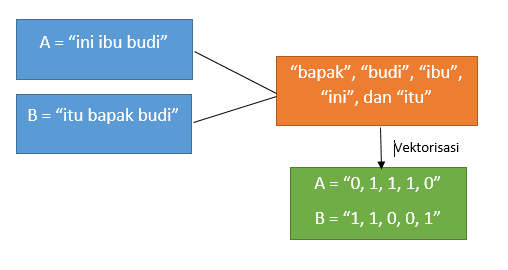
\includegraphics[width=4cm]{figures/1174054/5/1.png}
		\centering
		\caption{Vektorisasi Teks}
	\end{figure}

\item Mengapa dimensi dari vektor dataset google bisa sampai 300\\
Dimensi dari vektor dataset google bisa sampai 300 disebabkan karena dalam satu dataset berisi setidaknya 3 milyar kata dan kalimat. Dimensi tersebut berisikan kata-kata yang unik sehingga dimensi pada dataset google bisa mencapai 300.
Contohnya, terdapat kata word dan earth pada dataset google tersebut setiap kata tersebut dibuat dimensi vektor 300 untuk kata word dan 300 dimensi vektor juga untuk kata earth lalu kata tersebut dibandingkan bobot kesamaan katanya maka akan muncul akurasi sekitar 70 persen kesamaan bobot dikarenakan kata word dan earth sama sama digunakan untuk kata benda.
\hfill\break
	\begin{figure}[H]
		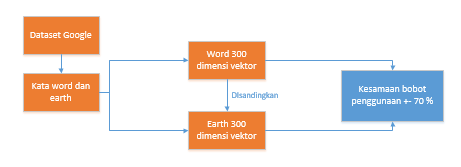
\includegraphics[width=4cm]{figures/1174054/5/2.png}
		\centering
		\caption{Dataset Google}
	\end{figure}

\item Konsep vektorisasi untuk kata\\
Vektorisasi untuk kata dengan mengetahui kata tengah dari suatu kalimat atau kata utama atau objek utama pada suatu kalimat. Contohnya seperti: jangan lupa untuk menjaga kesehatan di tengah wabah pandemik ini. kata tengah tersebut merupakan kesehatan yang memiliki bobot sebagai kata tengah dari suatu kalimat atau objek dari suatu kalimat. hal tersebut sangat berkaitan dengan dimensi vektor pada dataset google yang 300 tadi karena untuk mendapatkan nilai atau bobot dari kata tengah tersebut didapatkan dari proses dimensiasi dari kata tersebut.
\hfill\break
	\begin{figure}[H]
		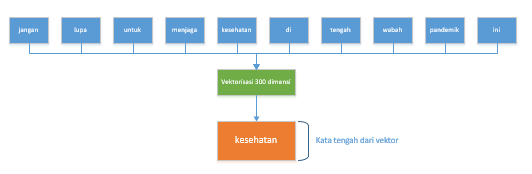
\includegraphics[width=4cm]{figures/1174054/5/3.png}
		\centering
		\caption{Vektorisasi untuk kata}
	\end{figure}

\item Konsep Vektorisasi untuk dokumen\\
Konsep vektorisasi untuk dokumen hampir sama seperti vektorisasi untuk kata hanya saja pemilihan katanya digunakan untuk mencari kesamaan atau memprediksi seberapa sering kemunculan kata dalam kalimat atau paragraf.
contohnya misalnya dalam sebuah artikel kita ingin mencari seberapa banyak kata saya muncul. maka dengan dengan doc2voc dapat diprediksi hasilnya.
\hfill\break
	\begin{figure}[H]
		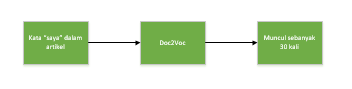
\includegraphics[width=4cm]{figures/1174054/5/4.png}
		\centering
		\caption{Vektorisasi untuk dokumen}
	\end{figure}

\item Mean dan Standar Deviasi\\
Mean merupakan suatu petunjuk terhadap kata-kata yang diolah jika kata kata itu memiliki akurasi yang tinggi berarti kata tersebut sering muncul begitu juga sebaliknya. 
Standar deviasi adalah standar untuk menimbang suatu kesalahan, sehingga kesalahan tersebut akan dianggap wajar misalnya ketika kita memperkirakan kedalaman dari dataset merupakan 2 atau 3 tapi pada kenyataanya merupakan 5 itu merupakan kesalahan tapi masih bisa dianggap wajar karena masih mendekati perkiraan awal.
\hfill\break
	\begin{figure}[H]
		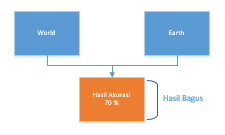
\includegraphics[width=4cm]{figures/1174054/5/5.png}
		\centering
		\caption{Mean dan Standar Deviasi}
	\end{figure}

\item Skip-gram\\
Skip-gram adalah salah satu teknik pembelajaran tanpa pengawasan yang digunakan untuk menemukan kata yang paling terkait untuk kata yang diberikan.
Skip-gram digunakan untuk memprediksi kata konteks untuk kata target yang diberikan. Ini kebalikan dari algoritma CBOW. Di sini, kata target adalah input sedangkan kata konteks adalah output. Karena ada lebih dari satu kata konteks yang dapat diprediksi yang membuat masalah ini sulit.
\hfill\break
	\begin{figure}[H]
		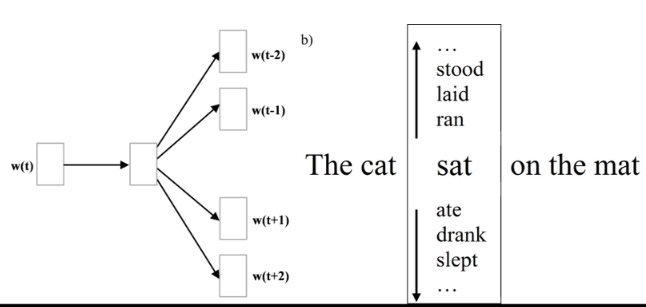
\includegraphics[width=4cm]{figures/1174054/5/6.png}
		\centering
		\caption{Skip-gram}
	\end{figure}

\end{enumerate}

\subsection{Praktek}
\begin{enumerate}
\item Nomor 1
\lstinputlisting[firstline=9, lastline=11]{src/1174054/5/1174054.py}
Dalam kode diatas berfungsi untuk mengimport library gensim. Gensim berfungsi untuk melakukan pemodelan dengan dataset atau topik yang telah ditentukan. Dalam keluaran 100 logging library opsional karena logging hanya menampilkan berupa log untuk setiap code yang dijalankan. Dan dalam keluaran 101 tersebut hasilnya berupa vektor google. Untuk hasil dari program tersebut dapat dilihat pada gambar dibawah ini :
\hfill\break
	\begin{figure}[H]
		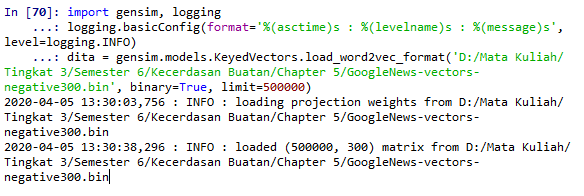
\includegraphics[width=4cm]{figures/1174054/5/7.png}
		\centering
		\caption{Hasil Nomor 1}
	\end{figure}
	
\lstinputlisting[firstline=13, lastline=14]{src/1174054/5/1174054.py}
Dalam kode diatas digunakan untuk menampilkan hasil vektorisasi data dari kata love. Untuk hasilnya dapat dilihat pada gambar berikut :
\hfill\break
	\begin{figure}[H]
		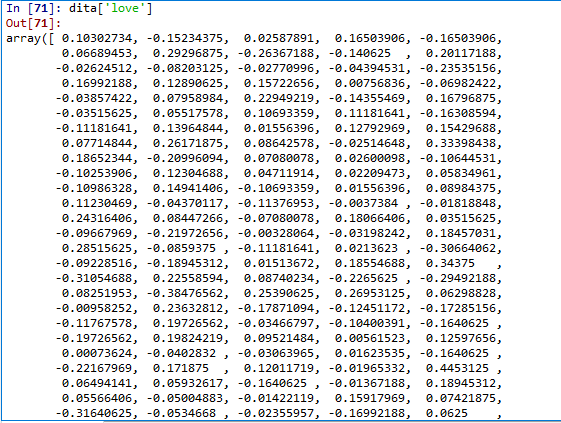
\includegraphics[width=4cm]{figures/1174054/5/8.png}
		\centering
		\caption{Hasil Nomor 1 - Love}
	\end{figure}

\lstinputlisting[firstline=15, lastline=16]{src/1174054/5/1174054.py}
Dalam kode diatas digunakan untuk menampilkan hasil vektorisasi data dari kata faith. Untuk hasilnya dapat dilihat pada gambar berikut :
\hfill\break
	\begin{figure}[H]
		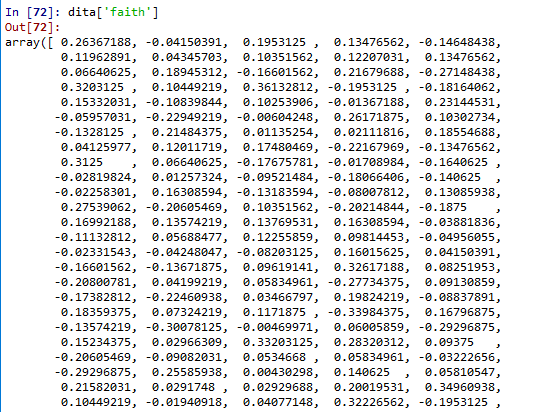
\includegraphics[width=4cm]{figures/1174054/5/9.png}
		\centering
		\caption{Hasil Nomor 1 - Faith}
	\end{figure}
	
\lstinputlisting[firstline=17, lastline=18]{src/1174054/5/1174054.py}
Dalam kode diatas digunakan untuk menampilkan hasil vektorisasi data dari kata fall. Untuk hasilnya dapat dilihat pada gambar berikut :
\hfill\break
	\begin{figure}[H]
		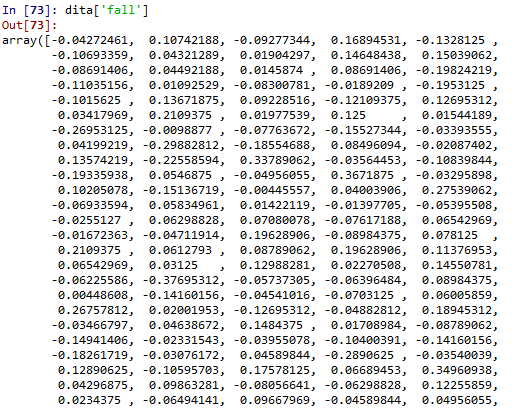
\includegraphics[width=4cm]{figures/1174054/5/10.png}
		\centering
		\caption{Hasil Nomor 1 - Fall}
	\end{figure}
	
\lstinputlisting[firstline=19, lastline=20]{src/1174054/5/1174054.py}
Dalam kode diatas digunakan untuk menampilkan hasil vektorisasi data dari kata sick. Untuk hasilnya dapat dilihat pada gambar berikut :
\hfill\break
	\begin{figure}[H]
		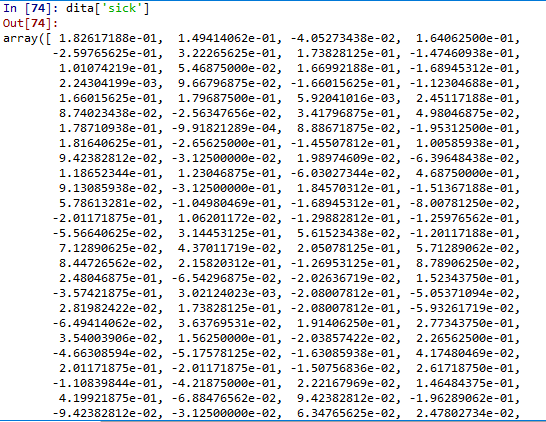
\includegraphics[width=4cm]{figures/1174054/5/11.png}
		\centering
		\caption{Hasil Nomor 1 - Sick}
	\end{figure}
	
\lstinputlisting[firstline=21, lastline=22]{src/1174054/5/1174054.py}
Dalam kode diatas digunakan untuk menampilkan hasil vektorisasi data dari kata clear. Untuk hasilnya dapat dilihat pada gambar berikut :
\hfill\break
	\begin{figure}[H]
		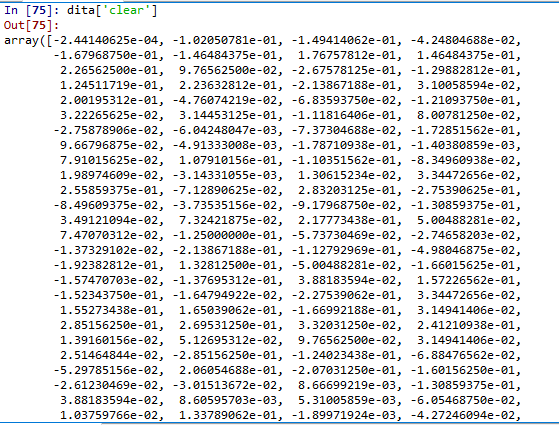
\includegraphics[width=4cm]{figures/1174054/5/12.png}
		\centering
		\caption{Hasil Nomor 1 - Clear}
	\end{figure}
	
\lstinputlisting[firstline=23, lastline=24]{src/1174054/5/1174054.py}
Dalam kode diatas digunakan untuk menampilkan hasil vektorisasi data dari kata shine. Untuk hasilnya dapat dilihat pada gambar berikut :
\hfill\break
	\begin{figure}[H]
		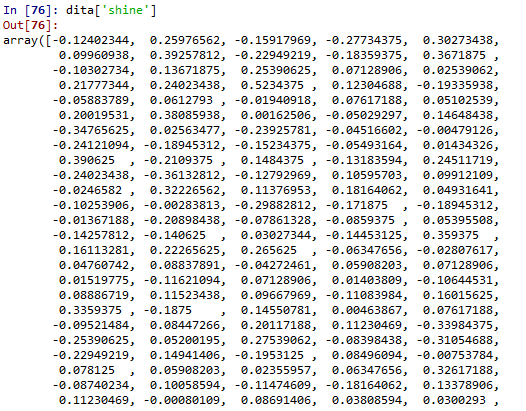
\includegraphics[width=4cm]{figures/1174054/5/13.png}
		\centering
		\caption{Hasil Nomor 1 - Shine}
	\end{figure}
	
\lstinputlisting[firstline=25, lastline=26]{src/1174054/5/1174054.py}
Dalam kode diatas digunakan untuk menampilkan hasil vektorisasi data dari kata bag. Untuk hasilnya dapat dilihat pada gambar berikut :
\hfill\break
	\begin{figure}[H]
		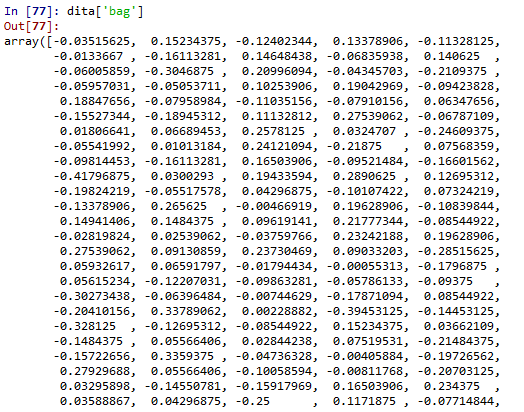
\includegraphics[width=4cm]{figures/1174054/5/14.png}
		\centering
		\caption{Hasil Nomor 1 - Bag}
	\end{figure}
	
\lstinputlisting[firstline=27, lastline=28]{src/1174054/5/1174054.py}
Dalam kode diatas digunakan untuk menampilkan hasil vektorisasi data dari kata car. Untuk hasilnya dapat dilihat pada gambar berikut :
\hfill\break
	\begin{figure}[H]
		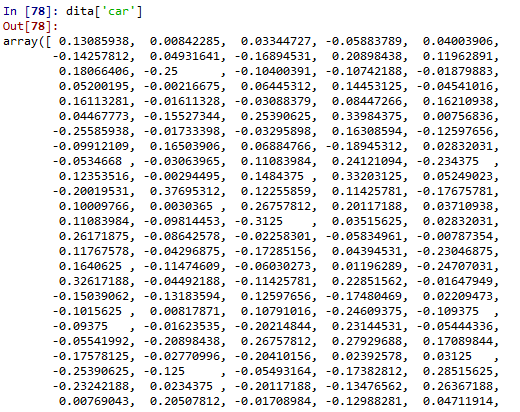
\includegraphics[width=4cm]{figures/1174054/5/15.png}
		\centering
		\caption{Hasil Nomor 1 - Car}
	\end{figure}
	
\lstinputlisting[firstline=29, lastline=30]{src/1174054/5/1174054.py}
Dalam kode diatas digunakan untuk menampilkan hasil vektorisasi data dari kata wash. Untuk hasilnya dapat dilihat pada gambar berikut :
\hfill\break
	\begin{figure}[H]
		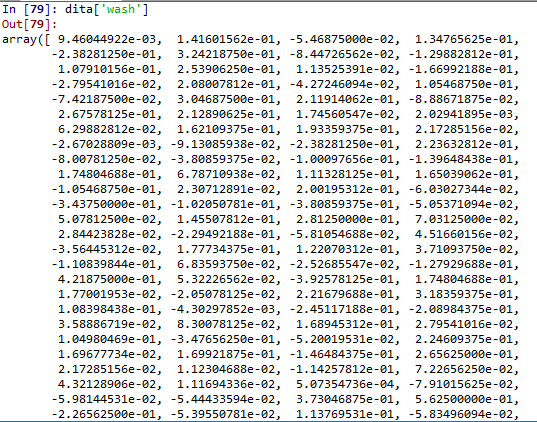
\includegraphics[width=4cm]{figures/1174054/5/16.png}
		\centering
		\caption{Hasil Nomor 1 - Wash}
	\end{figure}
	
\lstinputlisting[firstline=31, lastline=32]{src/1174054/5/1174054.py}
Dalam kode diatas digunakan untuk menampilkan hasil vektorisasi data dari kata motor. Untuk hasilnya dapat dilihat pada gambar berikut :
\hfill\break
	\begin{figure}[H]
		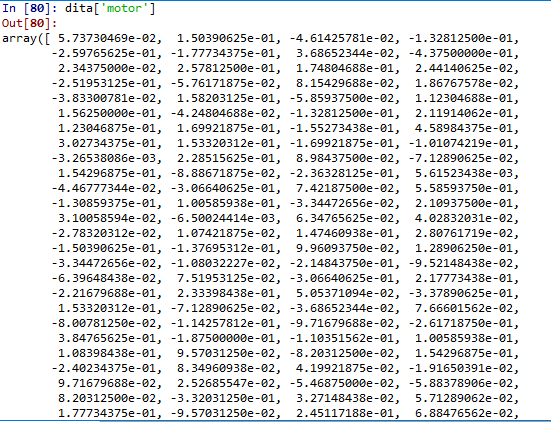
\includegraphics[width=4cm]{figures/1174054/5/17.png}
		\centering
		\caption{Hasil Nomor 1 - Motor}
	\end{figure}
	
\lstinputlisting[firstline=33, lastline=34]{src/1174054/5/1174054.py}
Dalam kode diatas digunakan untuk menampilkan hasil vektorisasi data dari kata cycle. Untuk hasilnya dapat dilihat pada gambar berikut :
\hfill\break
	\begin{figure}[H]
		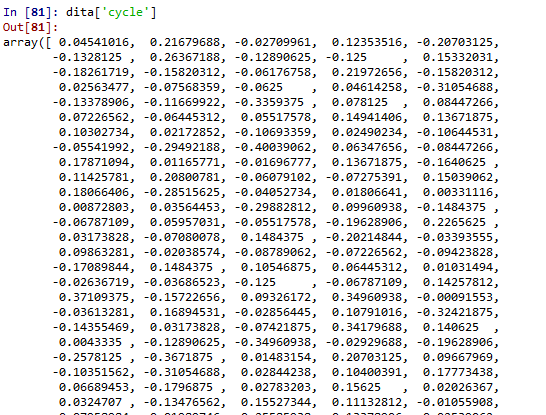
\includegraphics[width=4cm]{figures/1174054/5/18.png}
		\centering
		\caption{Hasil Nomor 1 - Cycle}
	\end{figure}
	
\lstinputlisting[firstline=35, lastline=36]{src/1174054/5/1174054.py}
Dalam kode diatas digunakan untuk persentase dari kata wash dan clear, persentase nya adalah 9 persen, hasil tersebut tidak terlalu baik. Untuk hasilnya dapat dilihat pada gambar berikut :
\hfill\break
	\begin{figure}[H]
		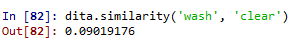
\includegraphics[width=4cm]{figures/1174054/5/19.png}
		\centering
		\caption{Hasil Nomor 1 - Wash dan Clear}
	\end{figure}

\lstinputlisting[firstline=37, lastline=38]{src/1174054/5/1174054.py}
Dalam kode diatas digunakan untuk persentase dari kata bag dan love, persentase nya adalah 7 persen, hasil tersebut tidak terlalu baik. Untuk hasilnya dapat dilihat pada gambar berikut :
\hfill\break
	\begin{figure}[H]
		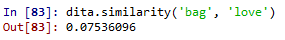
\includegraphics[width=4cm]{figures/1174054/5/20.png}
		\centering
		\caption{Hasil Nomor 1 - Bag dan Love}
	\end{figure}
	
\lstinputlisting[firstline=39, lastline=40]{src/1174054/5/1174054.py}
Dalam kode diatas digunakan untuk persentase dari kata motor dan car, persentase nya adalah 48 persen, hasil tersebut cukup baik karena mesin dapat membedakan antara motor dan car. Untuk hasilnya dapat dilihat pada gambar berikut :
\hfill\break
	\begin{figure}[H]
		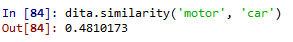
\includegraphics[width=4cm]{figures/1174054/5/21.png}
		\centering
		\caption{Hasil Nomor 1 - Motor dan Car}
	\end{figure}
	
\lstinputlisting[firstline=41, lastline=42]{src/1174054/5/1174054.py}
Dalam kode diatas digunakan untuk persentase dari kata sick dan faith, persentase nya adalah 12 persen, hasil tersebut cukup baik. Untuk hasilnya dapat dilihat pada gambar berikut :
\hfill\break
	\begin{figure}[H]
		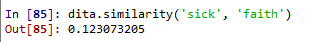
\includegraphics[width=4cm]{figures/1174054/5/22.png}
		\centering
		\caption{Hasil Nomor 1 - Sick dan Faith}
	\end{figure}
	
\lstinputlisting[firstline=43, lastline=44]{src/1174054/5/1174054.py}
Dalam kode diatas digunakan untuk persentase dari kata cycle dan shine, persentase nya adalah 6 persen, hasil tersebut kurang baik. Untuk hasilnya dapat dilihat pada gambar berikut :
\hfill\break
	\begin{figure}[H]
		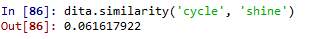
\includegraphics[width=4cm]{figures/1174054/5/23.png}
		\centering
		\caption{Hasil Nomor 1 - Cycle dan Shine}
	\end{figure}

\item Nomor 2
\hfill\break
	\lstinputlisting[firstline=47, lastline=51]{src/1174054/5/1174054.py}
Kode diatas digunakan untuk membuat string dengan meenggunakan library re, didalamnya dapat digunakan test string sebagai string dan membuat print untuk menambahkan kalimat sebelum test string. Untuk hasilnya dapat dilihat pada gambar berikut :
\hfill\break
	\begin{figure}[H]
		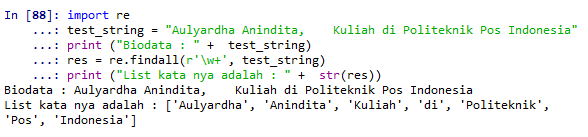
\includegraphics[width=4cm]{figures/1174054/5/24.png}
		\centering
		\caption{Hasil Nomor 2 - 1}
	\end{figure}
	
\hfill\break
	\lstinputlisting[firstline=53, lastline=62]{src/1174054/5/1174054.py}
Kode diatas digunakan untuk membuat string dengan memakai library random, yaitu dengan memakai sent matrix untuk membuat string dan untuk result sebagai print random yang akan diacak. Hasilnya dapat dilihat pada gambar berikut :
\hfill\break
	\begin{figure}[H]
		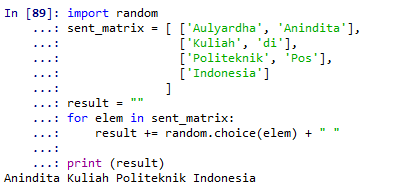
\includegraphics[width=4cm]{figures/1174054/5/25.png}
		\centering
		\caption{Hasil Nomor 2 - 2}
	\end{figure}
	
\item Nomor 3
\hfill\break
	\lstinputlisting[firstline=75, lastline=98]{src/1174054/5/1174054.py}
Kode diatas digunakan untuk mengimport library gensim. library gensim biasanya digunakan untuk pemodelan topik tanpa pengawasan dan pemrosesan bahasa alami, atau bisa juga disebut dengan unsupervised. fungsi dari doc2vec adalah untuk membandingkan bobot data yang terdapat pada dokumen lainnya, apakah kata-kata didalamnya sama atau tida. Sedangkan untuk tagged document digunakan untuk memasukkan kata-kata pada setiap dokumen untuk divektorisasi, dam model untuk membuat model dan save file model. Untuk hasilnya dapat dilihat pada gambar berikut :
\hfill\break
	\begin{figure}[H]
		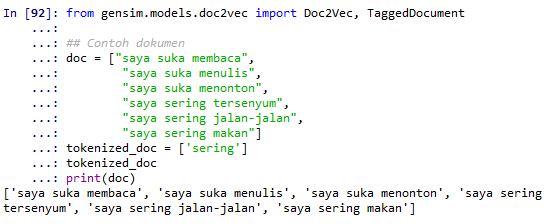
\includegraphics[width=4cm]{figures/1174054/5/26.png}
		\centering
		\caption{Hasil Nomor 3-1}
	\end{figure}
	\begin{figure}[H]
		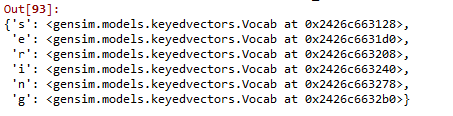
\includegraphics[width=4cm]{figures/1174054/5/27.png}
		\centering
		\caption{Hasil Nomor 3-2}
	\end{figure}
	
\item Nomor 4
\hfill\break
	\lstinputlisting[firstline=101, lastline=111]{src/1174054/5/1174054.py}
Dalam kode diatas saya menggunakan dataset dari acllmdb. untuk menambahkan data training kita bisa mengimport library os agar os sendiri dapat melakukan interaksi dengan python. kemudian saya membuat variable unsup sentences. Lalu pilih direktori tempat data kita disimpan. Selanjutnya kita bisa menyortir data yang terdapat pada folder acllmdb dan membaca file tersebut dengan ekstensi .txt. Hasilnya dapat dilihat pada gambar berikut:
\hfill\break
	\begin{figure}[H]
		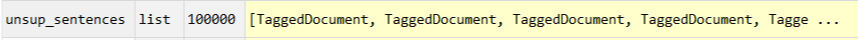
\includegraphics[width=4cm]{figures/1174054/5/28.png}
		\centering
		\caption{Hasil Nomor 4}
	\end{figure}	

\item Nomor 5
\hfill\break
	\lstinputlisting[firstline=114, lastline=116]{src/1174054/5/1174054.py}
Dalam kode diatas pada bagian mengacak data digunakan untuk mengacak data agar ketika data dirunning mampu berjalan dengan baik dan hasil persentase nya juga lebih baik. Dan untuk pembersihan data digunakan untuk memberikan ruang bagi ram laptop setelah melakukan running data sebanyak 3 juta lebih. Untuk hasilnya dapat dilihat pada gambar berikut :
\hfill\break
	\begin{figure}[H]
		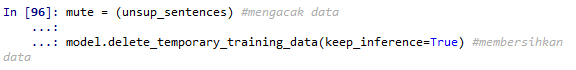
\includegraphics[width=4cm]{figures/1174054/5/29.png}
		\centering
		\caption{Hasil Nomor 5}
	\end{figure}
	
\item Nomor 6\\
\hfill\break
	\lstinputlisting[firstline=120, lastline=122]{src/1174054/5/1174054.py}
Dalam kode diatas terdapat save data yang digunakan untuk menyimpan file hasil dari proses training sebelumnya. Model tersebut dilakukan penyimpanan untuk memberikan keringanan pada ram agar ketika akan melakukan pelatihan lagi, model tersebut tinggal di load saja tanpa harus melakukan pelatihan dari awal sehingga bisa menghemat waktu. Sedangkan pada delete temporart digunakan untuk menghapus data latihan sebelumnya yang sudah dilakukan dan disimpan yang memiliki tujuan untuk memberikan keringanan pada ram. Untuk hasilnya dpat dilihat pada gambar berikut :
\hfill\break
	\begin{figure}[H]
		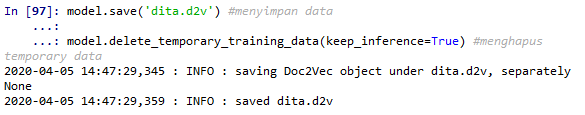
\includegraphics[width=4cm]{figures/1174054/5/30.png}
		\centering
		\caption{Hasil Nomor 6}
	\end{figure}
	
\item Nomor 7
\hfill\break
	\lstinputlisting[firstline=125, lastline=127]{src/1174054/5/1174054.py}
Dalam kode diatas terdapat infer vector yang digunakan untuk membandingkan kata yang tercantum dengan vektor yang mana pada dokumen yang sudah diload pada step sebelumnya. selain itu, infer vector juga digunakan untuk menghitung atau mengkalkulasikan vektor dari kata yang dicantumkan dari model yang telah dibuat. Hasilnya dapat dilihat pada gambar dibawah ini :
\hfill\break
	\begin{figure}[H]
		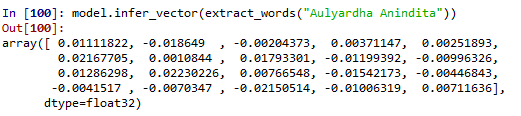
\includegraphics[width=4cm]{figures/1174054/5/31.png}
		\centering
		\caption{Hasil Nomor 7}
	\end{figure}
	
\item Nomor 8
\hfill\break
	\lstinputlisting[firstline=130, lastline=133]{src/1174054/5/1174054.py}
Pada kode diatas terdapat cosine similary yang biasanya digunakan untuk membandingkan vektorisasi data diantara dua kata yang diinputkan, jika hasil persentase dari keuda data tersebut lebih dari 50 persen, hal itu memungkinkan kata tersebut tidak terdapat dalam satu file. hasilnya dapat didapatkan pada code tersebut hanya 0,8 persen hal itu dikarenakan kata pertama dan kedua tidak memiliki kesamaan vektorisasi dan tidak terdapat pada salah satu dokumen. untuk hasilnya dapat dilihat pada gambar berikut :
\hfill\break
	\begin{figure}[H]
		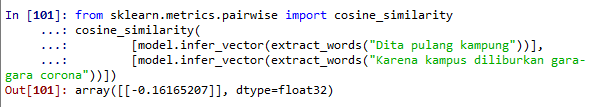
\includegraphics[width=4cm]{figures/1174054/5/32.png}
		\centering
		\caption{Hasil Nomor 8}
	\end{figure}
	
\item Nomor 9
\hfill\break
	\lstinputlisting[firstline=137, lastline=143]{src/1174054/5/1174054.py}
Pada kode diatas digunakan untuk melakukan perhitungan persentase dengan menggunakan cross validation dengan metode kneighborsClassifier. untuk hasilnya dapat dilihat pada gambar berikut :
\hfill\break
	\begin{figure}[H]
		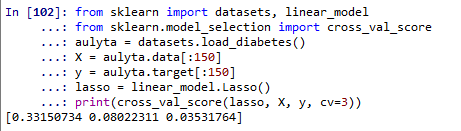
\includegraphics[width=4cm]{figures/1174054/5/33.png}
		\centering
		\caption{Hasil Nomor 9}
	\end{figure}
\end{enumerate}

\subsection{Penanganan Error}
\begin{enumerate}
\item ScreenShoot Error
	\begin{figure}[H]
		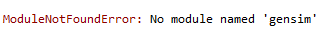
\includegraphics[width=4cm]{figures/1174054/5/error2.png}
		\centering
		\caption{Module Not Found Error}
	\end{figure}
	\begin{figure}[H]
		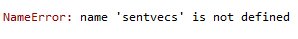
\includegraphics[width=4cm]{figures/1174054/5/error1.png}
		\centering
		\caption{Name Error}
	\end{figure}

	\item Tuliskan Kode Error dan Jenis Error
	\begin{itemize}
		\item Module Not Found Error
		\item Name Error

	\end{itemize}
	\item Cara Penanganan Error
	\begin{itemize}
		\item File Not Found Error
		\hfill\break
		Error terjadi karena belum menginstal package atau library gensim. Untuk mengatasinya dengan mengisntal library gensim pada anaconda
		\item Name Error
		\hfill\break
		Error terjadi karena sentvcs tidak terdefinisi. Untuk mengatasinya yaitu dengan membuat variabel baru dengan nama yang sama.
	\end{itemize}
\end{enumerate}


\subsection{Bukti Tidak Plagiat}
\begin{figure}[H]
	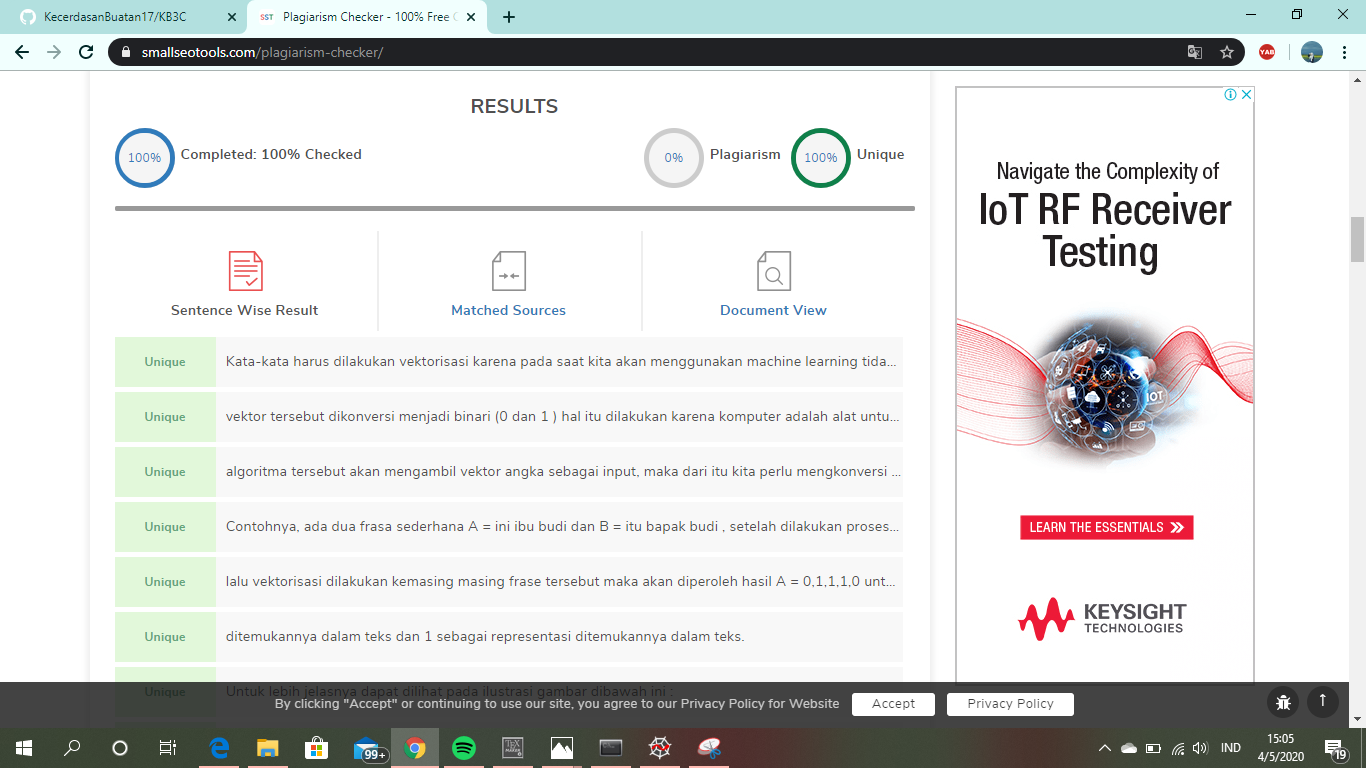
\includegraphics[width=4cm]{figures/1174054/5/plagiarisme.png}
	\centering
	\caption{Bukti Plagiasrisme}
\end{figure}

\subsection{Link Youtube}
https://youtu.be/2YUr0IwEu-w